Memory Allocation
Java memory management has concepts 



Memory Deallocation
Garbage Collection (GC) is a Java memory management method performed by JVM. 
GC tracks the state of objects on Java heap and triggers removal of unreferenced objects from memory. 

The Java heap structure is shown in Figure. It can be separated into three main parts where store objects for each corresponding generation: 
permanent generation, young generation, and old generation. The region for permanent generation stores metadata required by JVM to describe 
class and method used in application which will be permanently lived on the region of memory. 

The young generation of Java heap contains new objects allocated and aged. When the young generation fills up, this triggers minor GC. 
All of unreferenced objects will be removed from Java heap and remained objects will be aged and eventually promoted to the old generation.

The old generation is used to store long survived objects. Typically, a threshold is set for young generation object and when the age is met, 
the object will be moved to the old generation. Eventually, the old generation object also needs to be removed when the object is unreferenced. 
This is called major GC. The process of generational GC is shown in Figure.

\begin{figure}[htb]
    \includegraphics[width=15cm]{java_heap.eps}
    \caption{Java Heap Structure}
    \label{fig:Sampling}
\end{figure}

\begin{figure}[htb]
    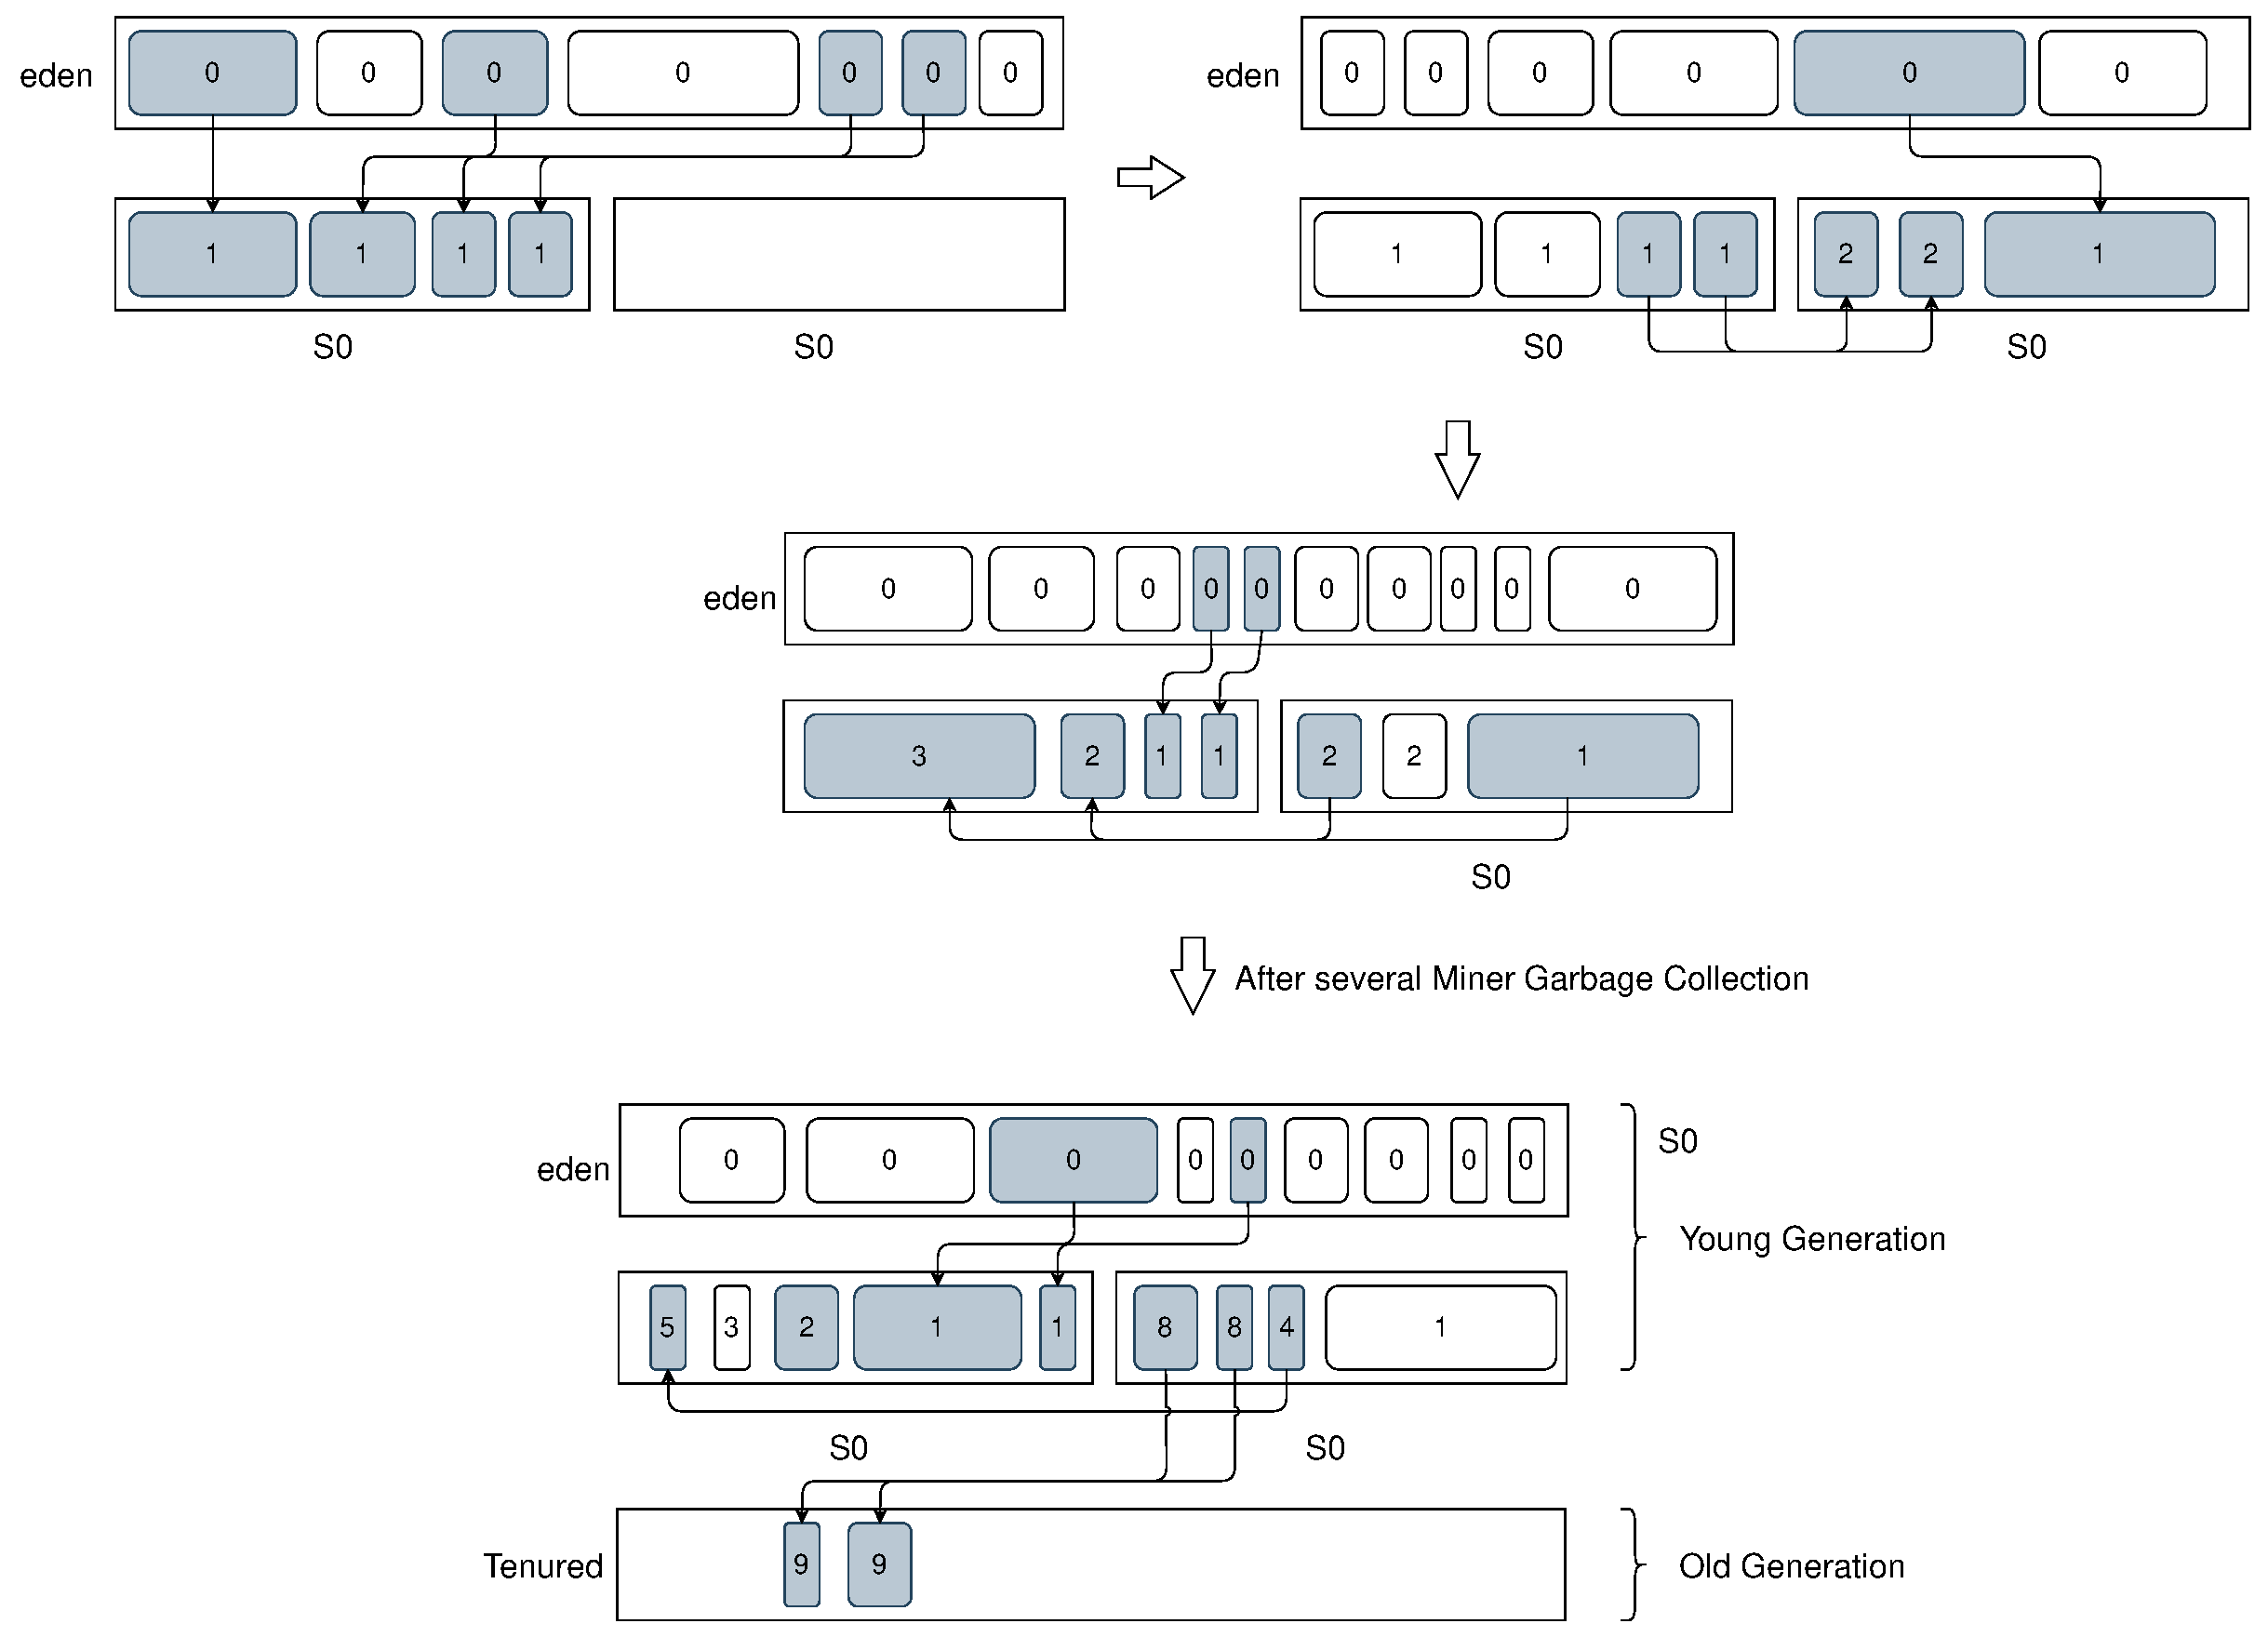
\includegraphics[width=15cm]{java_gc.eps}
    \caption{Java Garbage Collection}
    \label{fig:Sampling}
\end{figure}